\chapter{分类器设计}

\section{常用的分类技术}
\label{4.1}

\subsection{支持向量机方法}

支持向量机(Support Vector Machine,SVM)~\cite{cortes1995support}是一种有监督的统计学习方法,能够最小化经验误差和最大化几何边缘,被称为最大间隔分类器,可用于分类与回归分析。SVM的基本原理是在高维空间中寻找一个分类超平面,将不同类别的数据样本点分开,使不同类别的点之间的间隔最大,该分类超平面即为最大间隔超平面,对应的分类器称为最大间隔分类器。针对二分类问题,图~\ref{fig: svm}可以直观地描述SVM的空间特征。

\begin{figure}[!ht]
 \centering
 \includegraphics[width=4in]{svm.png}
\caption{SVM的训练数据样本及空间特征}
\label{fig: svm}
\end{figure}

假设数据样本为$x_1, x_2, \ldots, x_n$,分类超平面可以表达为:
\begin{equation}
w_Tx - b = 0 
\end{equation}

其中,$x$为分类超平面上的点;$w$为垂直于分类超平面的向量;$b$为位移量,用于改善分类超平面的灵活性,超平面不用必须通过原点。

两个分类超平面之间具有最大间隔,需要知道训练样本中的支撑向量、距离支撑向量最近的平行超平面,这些平行超平面可以表示为:
\begin{align}
\left\{ \begin{array}{l}
w^T x - b = 1\\
w^T x - b = -1
\end{array} \right.
\end{align}

其中,$w$是分类超平面的法向量,长度未定;1和-1只是为了计算方便而取的常量,其他常量只要互为相反数亦可。

如果给定的训练样本是线性可分的,那么就可以找到两个间距最大的平行超平面,并且这两个超平面之间没有任何训练样本,它们之间的距离为$2/||w||^2$。所以最小化$||w||^2$,就可以使这两个超平面之间的间隔最大化。
\begin{align}
min \; \frac{1}{2}||w||^2\\
s.t.\; y_i(w^Tx_i + b) \ge 1
\end{align}

通过将目标函数转化,求解SVM可以变成一个标准的凸优化问题。因为目标函数是二次的,而约束条件是线性的,所以这是一个凸二次规划问题。虽然这个问题是一个标准的二次规划问题,但同时具有它的特殊结构,通过将此二次规划问题转化为其对偶问题,可以找到更加有效的方法进行求解。整个对偶问题可表示为:
\begin{align}
\max_a\sum_{i = 1}^n\alpha_i - \frac{1}{2}\sum_{i, j = 1}^n\alpha_i\alpha_j y_i y_j < x_i \cdot x_j >\\
s.t. \; 0 \le \alpha_i \le C, i = 1, \ldots, n \\
\sum_{i =1}^n\alpha_i y_i = 0
\end{align}
其中,$\alpha$为引入的拉格朗日乘子。经计算,最优权值向量$w^*$和最优偏置$b^*$分别为
\begin{align}
w^* = \sum_{i= 1}^n \alpha_i^*y_i x_i \\
b^* = y_i - \sum_{i = 1}^n y_i \alpha_i^*(x_i \cdot x_j)
\end{align}
其中,$i\in \{ i|\alpha_i^* > 0\}$。因此得到最优分类面$(w^* \cdot x) + b^* = 0$,而最优分类函数为
\begin{align}
f(x) = sgn\{(w^* \cdot x) + b^*\} = sgn\{(\sum_{i = 1}^n\alpha_i^*y_i(x_i \cdot x_j)) + b^*\}
\end{align}

\subsection{随机森林方法}

在介绍随机森林方法之前,首先介绍决策树的概念,决策树是一种树,树中每个节点用于表示某个对象,每个分叉路径用于代表某个可能的属性值,从根节点到某叶节点所经历的路径所表示的对象值则对应该叶节点。

为了提高识别精度,必须要通过某种衡量准则选择特征,使得分割后的数据集的标签信息增益最大。信息增益是用于衡量给定属性区分训练样本能力的度量值,它的求解是用原始数据集标签熵减去分割后的数据集标签熵,如果熵变小了,则信息增益变大,表示给定属性对数据集的分类带来了一定的信息量。熵是信息论中广泛使用的一个度量标准,用于表示一件事情的不确定性,当要搞明白一件事所要求的信息量越高,这件事的不确定性越大,因而熵越大。假设$S$是包含关于某个目标概念的样本集,目标属性具有$m$个不同的种类,那么$S$相对于这$m$个状态类别的熵定义为:
\begin{align}
Entropy(S) = \sum_{i = 1}^m -p_i log_2 p_i
\end{align}
其中,$p_i$为$S$中不同类别样本的比例。

一个属性的信息增益可以看作由于使用这个属性分割样本从而导致的期望熵降低,一个属性$A$相对样本集合$S$的信息增益$Gain(S, A)$计算公式为:
\begin{align}
Gain(S, A) = Entropy(S) - \sum_{v\in V(A)} \frac{|S_v|}{|S|} Entropy(S_v)
\end{align}
其中,$V(A)$是属性$A$的值域,$S$是样本集合,$S_v$是$S$在属性$A$上值等于$v$的样本集合。

整个处理流程如下:首先计算每个属性的信息增益,然后依照信息增益最大原则选取属性,作为分割样本的属性。接着构建决策树,采用递归思想依次分割下去,直到执行完成就构建好了决策树。最后依据决策树进行分类,给出序列化决策树。

随机森林是一种采用决策树作为作为基预测器的集成学习方法,2001年由Breiman提出~\cite{breiman2001random},通过自助重采样技术,从总数量为$N$的原始训练样本集中有放回地重复随机选取$N$个样本,由此得到一个自助训练数据集,按此方法重复得到一组自助训练数据集。对每个自助训练集,用决策树学习方法(如C4.5、ID3、CART算法)创建一颗完全生长的无剪枝处理的决策树,进而得到一组决策树的集合。

对每个节点按固定概率分布来随机选择数目固定为$m$的特征(假设训练样本的总特征数目为$M$,$m << M$),作为在该节点寻找最佳分裂的依据。在预测时,根据所有决策树对新数据预测结果的平均值或根据投票多少来决定。

\subsection{极限学习机方法}

极限学习机(Extreme Learning Machine, ELM)是一种新型神经网络算法,最早是由新加坡南洋理工大学的黄广斌教授于2004年提出来的~\cite{huang2004extreme}。极限学习机的前身是单隐藏层反馈神经网络,在此基础上加上了一种新型的快速学习算法,使得学习速度得到了很大程度的提高。

神经网络的最小单位为“神经元”,一个最简单的神经网络可以仅仅由一个“神经元”组成,如图~\ref{fig: neuron}所示。

\begin{figure}
\centering
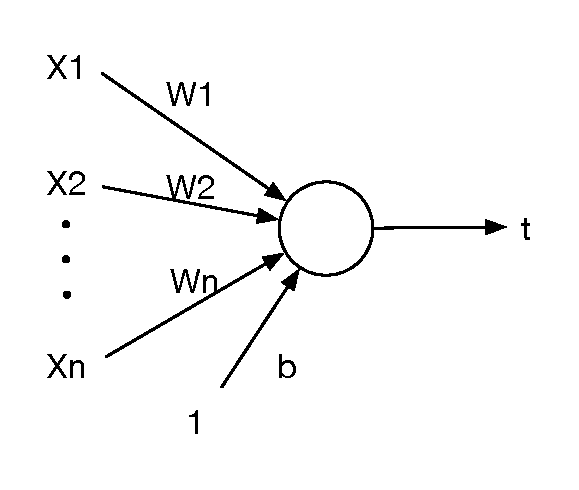
\includegraphics[width=0.3\linewidth]{neuron.eps}
\caption{单隐藏层反馈神经网络}
\label{fig: neuron}
\end{figure}

其中,第一列为输入向量,“1”表示截距,$b$表示偏置,箭头上的w为买个输入向量分量对应的权重值,最右端为输出。其输入-输出关系用数学公式表示为$y = g(w \cdot x + b)$,其中函数$g$叫做“激励函数”,通常采用sigmoid函数或tanh函数,这两个函数的表达式分别如下:
\begin{align}
g(z) = \frac{1}{1+exp(-z)}\\
g(z) = \frac{e^z - e^{-z}}{e^z + e^{-z}}
\end{align}
它们对应的图像分布见图~\ref{fig: sigmoid_tanh}。

\begin{figure}
\centering
\includegraphics[width=0.5\linewidth]{sigmoid_tanh.png}
\caption{sigmoid和tanh函数的图像}
\label{fig: sigmoid_tanh}
\end{figure}

可以看出,这两个函数都是逻辑函数,因而这里的输入-输出关系是一种逻辑回归。

稍微复杂一点的神经网络是联结不只一个的神经元,常见的三层神经网络(单隐藏层反馈神经网络)如图~\ref{fig: ELM-network}所示。

\begin{figure}
\centering
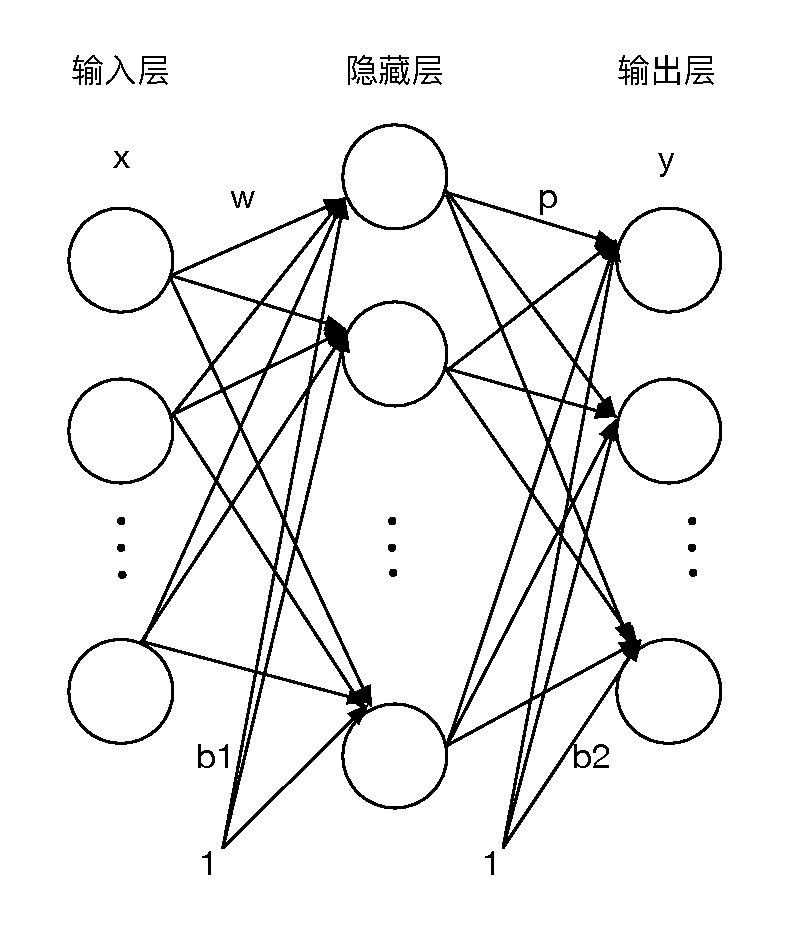
\includegraphics[width=0.5\linewidth]{Neural-network.eps}
\caption{单隐藏层反馈神经网络}
\label{fig: Neural-network}
\end{figure}

其中最左边一层叫做输入层,中间的一层叫做隐藏层,最右边一层叫做输出层。只有输入层和输出层可以跟外界进行联系,而隐藏层中的内容就对应一个黑盒子,外界无法观测到其值。从左往右来看,左边一层的输出总是连接着右边一层的输入,因而输出层第$k$个神经元的响应可以表示为:
\begin{align}
y[k] = [g(w_1 \cdot x + b_1) \cdot g(w_2 \cdot x + b_2) \cdot \ldots \cdot g(w_L \cdot x + b_L)] \cdot p_k + b_2[k], \; k = 1, \ldots, m
\end{align}
其中,$w_i$是一个向量,表示隐藏层第$i$个神经元的输入权重,$p_i$也是一个向量,表示输出层第$k$个神经元的输入权重。

单隐藏层反馈神经网络的主要优点为:1)可以充分拟合出任何复杂的输入-输出关系;2)每一层中单个的神经元以及一条连接对整个神经网络的作用是很小的,当少量神经元和连接发生错误时,对整个网络的影响不大,这样就增强了网络的容错性。其缺点是学习速度较慢,在时间消耗上远高于我们所能接受的最多时间。为了解决这一问题,很多研究者对单隐藏层反馈神经网络进行了进一步的探索,从而在运行时间上有了改进。

黄广斌教授通过对单隐藏层反馈神经网络的进一步研究发现,当“激励函数”$g$能够在任何一个区间内都满足无限可微的条件时,我们就可以随机地生成$w_i$和$b_i$的值,不用对它们进一步调整了。并且 在某种情况下$||T - Hp||_F = 0$一式是成立的,因而输出层的偏置也就可以忽略了。这样就可以得到一个新的单隐藏层反馈神经网络,叫做极限学习机网络,如图~\ref{fig: ELM-network}所示。
\begin{figure}
\centering
\includegraphics[width=0.5\linewidth]{ELM-network.eps}
\caption{极限学习机网络}
\label{fig: ELM-network}
\end{figure}

与单隐藏层反馈神经网络相比,极限学习机具有以下几个优点:
\begin{enumerate}
\item 忽略了输出层偏置,并且通过随机的方式产生隐藏层的偏置和输入层的权重,需要计算的就只剩下输出层的权重了。比单隐藏反馈网络要求解的内容少了很多,因而学习时间大大降低。在实际实验中,采用极限学习机算法进行训练通常几秒就完成了,而用单隐藏层神经网络进行训练往往需要几十甚至几百倍的时间。
\item 泛化能力更强。
\item 避免了所求解的局部最优问题以及过拟合的问题。
\end{enumerate}

\section{分类算法选择}

目前分类算法有很多种,而对于挑选出来的三类特征,我们将通过具体实验来选出适用每一类特征的分类算法。从论文~\cite{gorsky2010digital}中,我们知道对PkID中的特征,采用随机森林分类算法的分类准确率最高,因而对于我们挑选出的PkID中的22个特征,随机森林算法也应该最适用。在图像处理和机器视觉领域,LBP特征一般使用支持向量机分类算法进行分类,内距离形状上下文一般使用极限学习机进行分类。下面通过具体实验来进行验证,对这三类特征分别用~\ref{4.1}节介绍的三种分类进行分类,从而选出其最适用的分类算法。

首先对于PkID中的22个特征用支持向量机、随机森林、极限学习机分类算法分别进行分类,对分类结果用$K$折交叉验证进行评价,结果是用随机森林算法分类效果最好,结果如表~\ref{22-Features-RF}所示,分类准确率达到73\%,错误率为21.9\%。

\begin{table}
\centering
\caption{PkID的22个特征采用随机森林进行分类的结果}
\begin{tabular}{c}
\includegraphics[width=1.0\linewidth]{22-Features-RF.pdf}
\end{tabular}
\label{22-Features-RF}
\end{table}

然后对训练集中图像提取LBP特征,并用支持向量机、随机森林、极限学习机分类算法分别进行训练,生成的分类器对测试集的分类结果中效果最好的是支持向量机,如表~\ref{LBP-SVM-2-folds-5-repetitions-32-256}所示,分类正确率为64\%,错误率为32.8\%。

\begin{table}
\centering
\caption{LBP特征采用支持向量机进行分类的结果}
\begin{tabular}{c}
\includegraphics[width=1.0\linewidth]{LBP-SVM-2-folds-5-repetitions-32-256.pdf}
\end{tabular}
\label{LBP-SVM-2-folds-5-repetitions-32-256}
\end{table}

最后,对内距离形状上下文特征进行实验,我们用到的数据集中一共有13个不同种类的浮游动物,其中同一类中的图像在形状方面也有可能相差较大,这是由于数据集中的类别有的是在“门”、“属”、“目”等不同级别,有的级别下面还包含很多子级,不同的子级之间有可能差别很多,所以在提取内距离形状上下文特征选取模板时,通常不能每类只选一幅图像作为模板,这样会导致该类下的某些子级被忽略了,不能被正确分类。经过实验,我们得出结论:当从每类浮游动物图像中选取3幅及以上的图像作为一类的模板时,分类效果会比较好。对于提取的内距离形状上下文特征,我们分别利用支持向量机、随机森林、极限学习机分类器进行训练并在测试集上验证,最终发现极限学习机分类算法最适用于这一特征。当对每一类选取的模板数目增多时,分类效果会有所提升,但同时学习速度也会变慢,两者成反比的关系。

对此,我们进行了一些实验作说明。当每类浮游动物图像中挑选3张作为模板,一共选取39幅时,采用ELM进行训练,在测试集上的分类结果评价如表~\ref{IDSC-39-Features-MATLAB-ELM},其分类准确率为59.4\%。选取65幅图像作为模板时,评价结果如表~\ref{IDSC-65-Features-MATLAB-ELM},其分类准确率为65\%。模板数目增加到104张时,评价结果如表~\ref{IDSC-104-Features-MATLAB-ELM},其分类准确率为65.6\%。可以看到,当模板数目增多时,分类准确率是有所提高的,但同时出现的问题是运行速度会下降很多,要在既保证分类准确率又保证运行效率的情况下设定最佳模板数目。而对内距离形状上下文特征使用支持向量机和随机森林分类算法时效果都没有极限学习机好。

上述三类实验验证了每类特征所对应有效的分类算法,至此,分类器设计完成。

\begin{table}
\centering
\caption{提取内距离形状上下文特征并采用极限学习机进行分类的结果(39张图像作为模板)}
\begin{tabular}{c}
\includegraphics[width=1.0\linewidth]{IDSC-39-Features-MATLAB-ELM.pdf}
\end{tabular}
\label{IDSC-39-Features-MATLAB-ELM}
\end{table}

\begin{table}
\centering
\caption{提取内距离形状上下文特征并采用极限学习机进行分类的结果(65张图像作为模板)}
\begin{tabular}{c}
\includegraphics[width=1.0\linewidth]{IDSC-65-Features-MATLAB-ELM.pdf}
\end{tabular}
\label{IDSC-65-Features-MATLAB-ELM}
\end{table}

\begin{table}
\centering
\caption{提取内距离形状上下文特征并采用极限学习机进行分类的结果(104张图像作为模板)}
\begin{tabular}{c}
\includegraphics[width=1.0\linewidth]{IDSC-104-Features-MATLAB-ELM.pdf}
\end{tabular}
\label{IDSC-104-Features-MATLAB-ELM}
\end{table}

